\documentclass[12pt,utf8,notheorems,compress,t]{beamer}
\usepackage{etex}

\usepackage{pgfpages}
\setbeameroption{show notes on second screen}
\setbeamertemplate{note page}[plain]
\newcommand{\jnote}[2]{\only<#1>{\note{\footnotesize\justifying#2\par}}}

% Workaround for the issue described at
% https://tex.stackexchange.com/questions/164406/beamer-using-href-in-notes.
\newcommand{\fixedhref}[2]{\makebox[0pt][l]{\hspace*{\paperwidth}\href{#1}{#2}}\href{#1}{#2}}

\usepackage[english]{babel}

\usepackage{mathtools}
\usepackage{booktabs}
\usepackage{stmaryrd}
\usepackage{array}
\usepackage{ragged2e}
\usepackage{multicol}
\usepackage{tabto}
\usepackage{xstring}
\usepackage{ifthen}
\usepackage{soul}\setul{0.3ex}{}
\usepackage[all]{xy}
\xyoption{rotate}
\usepackage{tikz}
\usetikzlibrary{mindmap,calc,shapes,shapes.callouts,shapes.arrows,patterns,fit,backgrounds,decorations.pathmorphing}
\hypersetup{colorlinks=false}

\usepackage{pifont}
\newcommand{\cmark}{\ding{51}}
\newcommand{\xmark}{\ding{55}}

\graphicspath{{images/}}

\usepackage[protrusion=true,expansion=true]{microtype}

\setlength\parskip{\medskipamount}
\setlength\parindent{0pt}

\title{How topos theory can help algebra and geometry}
\author{Ingo Blechschmidt}
\date{July 10th, 2018}

\useinnertheme[shadow=true]{rounded}
\useoutertheme[subsection=false]{miniframes}
\setbeamerfont{block title}{size={}}

\useinnertheme{rectangles}

\usecolortheme{orchid}
\usecolortheme{seahorse}
\definecolor{mypurple}{RGB}{150,0,255}
\setbeamercolor{structure}{fg=mypurple}
\definecolor{myred}{RGB}{150,0,0}
\setbeamercolor*{title}{bg=myred,fg=white}
\setbeamercolor*{titlelike}{bg=myred,fg=white}
\setbeamercolor{frame}{bg=black}

\usefonttheme{serif}
\usepackage[T1]{fontenc}
\usepackage{libertine}

\newcommand{\A}{\mathcal{A}}
\newcommand{\B}{\mathcal{B}}
\renewcommand{\AA}{\mathbb{A}}
\renewcommand{\C}{\mathcal{C}}
\newcommand{\E}{\mathcal{E}}
\newcommand{\F}{\mathcal{F}}
\newcommand{\M}{\mathcal{M}}
\renewcommand{\G}{\mathcal{G}}
\newcommand{\J}{\mathcal{J}}
\newcommand{\GG}{\mathbb{G}}
\renewcommand{\O}{\mathcal{O}}
\newcommand{\K}{\mathcal{K}}
\newcommand{\NN}{\mathbb{N}}
\newcommand{\QQ}{\mathbb{Q}}
\newcommand{\RR}{\mathbb{R}}
\newcommand{\CC}{\mathbb{C}}
\newcommand{\TT}{\mathbb{T}}
\newcommand{\PP}{\mathbb{P}}
\newcommand{\ZZ}{\mathbb{Z}}
\renewcommand{\P}{\mathcal{P}}
\newcommand{\aaa}{\mathfrak{a}}
\newcommand{\fff}{\mathfrak{f}}
\newcommand{\ppp}{\mathfrak{p}}
\newcommand{\mmm}{\mathfrak{m}}
\newcommand{\defeq}{\vcentcolon=}
\newcommand{\defeqv}{\vcentcolon\equiv}
\newcommand{\Sh}{\mathrm{Sh}}
\newcommand{\GL}{\mathrm{GL}}
\newcommand{\Zar}{\mathrm{Zar}}
\newcommand{\op}{\mathrm{op}}
\newcommand{\Set}{\mathrm{Set}}
\newcommand{\Ring}{\mathrm{Ring}}
\newcommand{\LocRing}{\mathrm{LocRing}}
\newcommand{\Eff}{\mathrm{Ef{}f}}
\newcommand{\Sch}{\mathrm{Sch}}
\newcommand{\Aff}{\mathrm{Aff}}
\newcommand{\LRS}{\mathrm{LRS}}
\newcommand{\Hom}{\mathrm{Hom}}
\newcommand{\Spec}{\mathrm{Spec}}
\newcommand{\lra}{\longrightarrow}
\newcommand{\RelSpec}{\operatorname{Spec}}
\renewcommand{\_}{\mathpunct{.}}
\newcommand{\?}{\,{:}\,}
\newcommand{\speak}[1]{\ulcorner\text{\textnormal{#1}}\urcorner}
\newcommand{\ull}[1]{\underline{#1}}
\newcommand{\affl}{\ensuremath{{\ull{\AA}^1}}}
\newcommand{\Ll}{\text{iff}}
\newcommand{\inv}{inv.\@}
\newcommand{\seq}{\vdash_{\!\!\!\vec x}}
\newcommand{\hg}{\mathbin{:}}  % homogeneous coordinates

\setbeamertemplate{blocks}[rounded][shadow=false]

% Adapted from https://latex.org/forum/viewtopic.php?t=2251 (Stefan Kottwitz)
\newenvironment<>{hilblock}{
  \begin{center}
    \begin{minipage}{9.85cm}
      \setlength{\textwidth}{9.85cm}
      \begin{actionenv}#1
        \def\insertblocktitle{}
        \par
        \usebeamertemplate{block begin}}{
        \par
        \usebeamertemplate{block end}
      \end{actionenv}
    \end{minipage}
  \end{center}}

\newcommand{\bignumber}[1]{
  \renewcommand{\insertenumlabel}{#1}\scalebox{1.5}{\usebeamertemplate{enumerate item}}
}

\newenvironment{indentblock}{%
  \list{}{\leftmargin\leftmargin}%
  \item\relax
}{%
  \endlist
}

\newcommand{\hcancel}[5]{%
  \tikz[baseline=(tocancel.base)]{
    \node[inner sep=0pt,outer sep=0pt] (tocancel) {#1};
    \draw[red, line width=0.4mm] ($(tocancel.south west)+(#2,#3)$) -- ($(tocancel.north east)+(#4,#5)$);
  }%
}

\newenvironment{changemargin}[2]{%
  \begin{list}{}{%
    \setlength{\topsep}{0pt}%
    \setlength{\leftmargin}{#1}%
    \setlength{\rightmargin}{#2}%
    \setlength{\listparindent}{\parindent}%
    \setlength{\itemindent}{\parindent}%
    \setlength{\parsep}{\parskip}%
  }%
  \item[]}{\end{list}}

\tikzset{
  invisible/.style={opacity=0,text opacity=0},
  visible on/.style={alt={#1{}{invisible}}},
  alt/.code args={<#1>#2#3}{%
    \alt<#1>{\pgfkeysalso{#2}}{\pgfkeysalso{#3}}}
}

\newcommand{\pointthis}[3]{%
  \tikz[remember picture,baseline]{
    \node[anchor=base,inner sep=0,outer sep=0] (#2) {#2};
    \node[visible on=#1,overlay,rectangle callout,rounded corners,callout relative pointer={(-0.1cm,0.5cm)},fill=blue!20] at ($(#2.north)+(-0.1cm,-1.1cm)$) {#3};
  }%
}

% Adapted from https://latex.org/forum/viewtopic.php?t=2251 (Stefan Kottwitz)
\newenvironment<>{varblock}[2]{
  \begin{center}
    \begin{minipage}{#1}
      %\setlength{\textwidth}{#1}
      \begin{actionenv}#3
  \def\insertblocktitle{\centering #2}
  \par
  \usebeamertemplate{block begin}}{
        \par
        \usebeamertemplate{block end}
      \end{actionenv}
    \end{minipage}
  \end{center}}

\setbeamertemplate{frametitle}{%
  \vskip0.7em%
  \leavevmode%
  \begin{beamercolorbox}[dp=1ex,center]{}%
      \usebeamercolor[fg]{item}{\textbf{{\Large \insertframetitle}}}
  \end{beamercolorbox}%
}

\setbeamertemplate{navigation symbols}{}

\newcounter{framenumberpreappendix}
\newcommand{\backupstart}{
  \setcounter{framenumberpreappendix}{\value{framenumber}}
}
\newcommand{\backupend}{
  \addtocounter{framenumberpreappendix}{-\value{framenumber}}
  \addtocounter{framenumber}{\value{framenumberpreappendix}}
}

\setbeamertemplate{footline}{%
  \begin{beamercolorbox}[wd=\paperwidth,ht=2.25ex,dp=1ex,right,rightskip=1mm,leftskip=1mm]{}%
    % \inserttitle
    \hfill
    \insertframenumber\,/\,\inserttotalframenumber
  \end{beamercolorbox}%
  \vskip0pt%
}


\newcommand{\hil}[1]{{\usebeamercolor[fg]{item}{\textbf{#1}}}}

\newcommand{\bad}[1]{\textcolor{red!90}{\textnormal{#1}}}


\begin{document}

\tikzstyle{topos} = [draw=mypurple, very thick, rectangle, rounded corners, inner sep=5pt, inner ysep=10pt]
\tikzstyle{title} = [fill=mypurple, text=white]

% Taken from Todd Lehman (CC-BY-SA) at https://tex.stackexchange.com/a/44920/32372

\newcommand{\setisprime}[1]{
  % Sets \isprime based on #1.
  \ifnum#1=1 \gdef\isprime{0} \else \gdef\isprime{1} \fi
  \foreach \sip in {2, 3,5,...,#1} {
    \pgfmathparse{\sip*\sip>#1? 1:0}
    \ifthenelse{\pgfmathresult=1}{
      % Early-out if \sip^2 > #1.
      \breakforeach
    }{
      % Otherwise test if \sip divides #1.
      \pgfmathparse{Mod(#1,\sip)==0? 1:0}
      \ifthenelse{\pgfmathresult=1}{
        \gdef\isprime{0}
        \breakforeach
      }{}
    }
  }
}

\newcommand{\setxy}[1]{
  % Sets \x and \y to loction of cell #1.
  \pgfmathtruncatemacro{\x}{Mod(#1-1,\cols)}
  \pgfmathtruncatemacro{\y}{(#1-1) / \cols}
  \pgfmathtruncatemacro{\y}{\cols - 1 - \y}
  \pgfmathparse{2.5*(\x+.5)}\let\x\pgfmathresult
  \pgfmathparse{2.5*(\y+.5)}\let\y\pgfmathresult
}

\newcommand{\numlabel}[2]{
  % Draws label #2 at cell #1.
  \setxy{\n}
  \node[fill=none, text=black] at (\x,\y) {#2};
}

\newcommand{\drawpolygon}[2]{
  % Draws polygon with #2 vertexes at cell #1.
  \setxy{#1}
  \ifthenelse{#2>1}{ % Polygon must have at least 2 sides.
    \ifthenelse{#2<30}{ % Draw polygon if it has a small number of sides.
      \filldraw (\x,\y) +(90:1)
      \foreach \drawi in {1,...,#2} {-- +(\drawi/#2*360+90:1)} -- cycle;
    }{ % Else approximate with circle.
      \filldraw (\x,\y) circle(1);
    }
  }{}
}

\newcommand{\setpolygoncolor}[1]{
  % Sets color based on #1.
  \gdef\polycolor{black}
  \ifnum#1=2\gdef\polycolor{black!50!white}\fi
  \ifnum#1=3\gdef\polycolor{yellow!95!red}\fi
  \ifnum#1=5\gdef\polycolor{yellow!0!red}\fi
  \ifnum#1=7\gdef\polycolor{blue!75!green}\fi
  \ifnum#1=11\gdef\polycolor{blue!70!red}\fi
  \ifnum#1=13\gdef\polycolor{blue!40!red}\fi
  \ifnum#1=17\gdef\polycolor{green!50!blue}\fi
  \ifnum#1=19\gdef\polycolor{green!80!black}\fi
  \ifnum#1=23\gdef\polycolor{green!50!red}\fi
  \ifnum#1=29\gdef\polycolor{yellow!50!black}\fi
  \ifnum#1=31\gdef\polycolor{orange!50!black}\fi
  \ifnum#1=37\gdef\polycolor{red!50!black}\fi
  \ifnum#1=41\gdef\polycolor{purple!50!black}\fi
  \ifnum#1=43\gdef\polycolor{blue!50!black}\fi
  \ifnum#1=47\gdef\polycolor{green!50!black}\fi
  \ifnum#1=53\gdef\polycolor{white!50!black}\fi
  \ifnum#1=59\gdef\polycolor{white!50!black}\fi
  \ifnum#1=61\gdef\polycolor{white!50!black}\fi
  \ifnum#1=67\gdef\polycolor{white!50!black}\fi
}

\newcommand{\sieve}[2]{
  \def\cols{#1}
  \def\rows{#2}
  \begin{tikzpicture}[scale=.5]
  \pgfmathtruncatemacro{\nmax}{\rows * \cols}

  \foreach \n in {1,...,\nmax} {
    \begin{scope}[fill=gray, fill opacity=.05,
                  draw=gray, draw opacity=.10,
                  line width=4]
      \drawpolygon{\n}{\n}
    \end{scope}
    \setisprime{\n}
    \ifthenelse{\isprime=1}{
      \numlabel{\n}{\bf\n}
    }{
      \def\startintensity{.33}
      \def\incrintensity{.10}
      \def\intensity{\startintensity}

      \def\m{\n}
      \pgfmathtruncatemacro{\i}{\m / 2}

      % Divide \m by \i until \m is extinguished.
      % Increment \i each time it does not divide into \m.
      \whiledo{\m>1}{
        \setisprime{\i}
        \pgfmathparse{Mod(\m,\i)==0? 1:0}
        \ifthenelse{\pgfmathresult=1\and\isprime=1}{
          \setpolygoncolor{\i}
          \begin{scope}[fill=\polycolor, fill opacity=\intensity,
                        draw=\polycolor!85!black, draw opacity=\intensity,
                        line width=\intensity*1.5]
            \drawpolygon{\n}{\i}
          \end{scope}
          \pgfmathtruncatemacro{\m}{\m / \i}
          \pgfmathparse{\intensity + \incrintensity}\let\intensity\pgfmathresult
        }{
          \pgfmathtruncatemacro{\i}{\i - 1}
          \def\intensity{\startintensity}
        }
      }
      \begin{scope}[text=black, text opacity=.5]
        \numlabel{\n}{\scriptsize\n}
      \end{scope}
    }
  }

  \end{tikzpicture}
}

\newcommand{\fakesieve}[2]{
  \def\cols{#1}
  \def\rows{#2}
  \begin{tikzpicture}[scale=.5,opacity=0]
  \pgfmathtruncatemacro{\nmax}{\rows * \cols}

  \foreach \n in {1,...,\nmax} {
    \begin{scope}[fill=gray,
                  draw=gray,
                  line width=4]
      \drawpolygon{\n}{\n}
    \end{scope}
    \setisprime{\n}
    \ifthenelse{\isprime=1}{
      \numlabel{\n}{\bf\n}
    }{
      \def\startintensity{.33}
      \def\incrintensity{.10}
      \def\intensity{\startintensity}

      \def\m{\n}
      \pgfmathtruncatemacro{\i}{\m / 2}

      % Divide \m by \i until \m is extinguished.
      % Increment \i each time it does not divide into \m.
      \whiledo{\m>1}{
        \setisprime{\i}
        \pgfmathparse{Mod(\m,\i)==0? 1:0}
        \ifthenelse{\pgfmathresult=1\and\isprime=1}{
          \setpolygoncolor{\i}
          \begin{scope}[fill=\polycolor,
                        draw=\polycolor!85!black,
                        line width=\intensity*1.5]
            \drawpolygon{\n}{\i}
          \end{scope}
          \pgfmathtruncatemacro{\m}{\m / \i}
          \pgfmathparse{\intensity + \incrintensity}\let\intensity\pgfmathresult
        }{
          \pgfmathtruncatemacro{\i}{\i - 1}
          \def\intensity{\startintensity}
        }
      }
      \begin{scope}[text=black]
        \numlabel{\n}{\scriptsize\n}
      \end{scope}
    }
  }

  \end{tikzpicture}
}

%\renewcommand{\sieve}[2]{SIEVE}
%\renewcommand{\fakesieve}[2]{SIEVE}

\newcommand{\drawbox}[4]{
  \node[topos, #4] [fit = #3] (#1) {};
  \node[title] at (#1.north) {#2};
}

\newcommand{\muchstuff}{
  \includegraphics[height=3em]{filmat}
  \scalebox{0.5}{\sieve{14}{2}}
}

\newcommand{\muchstuffplaceholder}{
  \includegraphics[height=3em]{filmat-placeholder}
  \scalebox{0.5}{\fakesieve{14}{2}}
}

\newcommand{\fewstuff}{
  \includegraphics[height=3em]{filmat}
  \scalebox{0.5}{\sieve{7}{2}}
}

\newcommand{\threeblobs}{
  \colorbox{mypurple}{\ \ }\quad
  \colorbox{mypurple}{\ \ }\quad
  \colorbox{mypurple}{\ \ }
}

\addtocounter{framenumber}{-1}

{\usebackgroundtemplate{\begin{minipage}{\paperwidth}\vspace*{4.95cm}\includegraphics[width=\paperwidth]{topos-horses}\end{minipage}}
\begin{frame}[c]
  \centering
  \medskip
  \hspace*{-3.9em}%

  \hil{How topos theory can help algebra and geometry} \\

  \emph{-- an invitation --}

  \vfill

  \scriptsize
  Ingo Blechschmidt \\
  July 10th, 2018
  \par
\end{frame}}

\begin{frame}{Toposes are \ldots}
  \begin{columns}
    \begin{column}{0.5\textwidth}
      \centering
      \hil{generalized spaces}
      \medskip

      \includegraphics[height=0.32\textwidth]{grothendieck}
      \quad
      \includegraphics[height=0.32\textwidth]{elliptic-curve}

      \footnotesize
      étale topos of a scheme \\
      field with one element
    \end{column}

    \begin{column}{0.5\textwidth}
      \centering
      \hil{mathematical universes}
      \medskip

      \begin{tikzpicture}
        \node (overview) {
          \scalebox{0.44}{\sieve{6}{4}}
        };
        \def\R{8pt}
        \begin{pgfonlayer}{background}
        \draw[decoration={bumps,segment length=8pt}, decorate, very thick, draw=mypurple]
          ($(overview.south west) + (\R, 0)$) arc(270:180:\R) --
          ($(overview.north west) + (0, -\R)$) arc(180:90:\R) --
          ($(overview.north east) + (-\R, 0)$) arc(90:0:\R) --
          ($(overview.south east) + (0, \R)$) arc(0:-90:\R) --
          cycle;
        \end{pgfonlayer}
      \end{tikzpicture}
    \end{column}
  \end{columns}

  \bigskip
  \bigskip

  \begin{columns}
    \begin{column}{0.5\textwidth}
      \centering
      \hil{categories of sheaves}
      \medskip

      \includegraphics[height=0.304\textwidth]{sheaf}

      \footnotesize
      A topos is a finitely complete cartesian closed category with a
      subobject classifier.
    \end{column}

    \begin{column}{0.5\textwidth}
      \centering
      \hil{embodiments of theories}
      \medskip

      \includegraphics[height=0.32\textwidth]{olivia-lattices}

      \footnotesize
      ``Let~$G$ be a group.''
    \end{column}
  \end{columns}

  \jnote{1}{Toposes were invented in the 1960s by Grothendieck in order to
  solve concrete problems in algebraic geometry. Their raison d'être is the
  following. In algebraic geometry, we want (and sometimes have to) work over
  fields other than~$\RR$ and~$\CC$ and even over arbitrary commutative rings.
  For the geometric objects in such settings, the \emph{schemes}, the Euclidean
  topology is not available; we have to make do with the \emph{Zariski
  topology}. However, important tools as singular cohomology don't work well
  with this topology (too few opens).

  The problem was solved by inventing \emph{étale topology} as an enhancement
  of the Zariski topology. However, contrary to its name, the étale topology
  isn't actually a topology in the usual sense. Putting the étale topology on a
  scheme doesn't yield a refined topological space, but a \emph{topos}.

  Toposes generalize topological spaces in two ways: Firstly, the ``open sets''
  of toposes don't actually have to be sets of points; they can be more general
  kinds of objects such as coverings. Toposes can even have no points at all
  and still be nontrivial (this is for instance the case for the \emph{topos of
  random sequences}). Secondly, while classically a given open
  subset is either contained in a further open subset or not, the opens of
  toposes can be contained in further opens in many different ways.
  % XXX: Link to Alex Simpson

  Recently, toposes are being used to help the mysterious field with
  one element come into being.}
  % XXX: Link to John Baez

  \jnote{2}{Since the 1960s, many more aspects of toposes were discovered.
  A popular reference on toposes starts with a list of 13 ways of viewing
  toposes.

  In this talk, we'll focus on the view of toposes as \emph{alternate
  mathematical universes}. We can do mathematics inside these alternate
  universes just as well as we can do mathematics inside the \emph{standard
  universe} (which is represented by a particular topos called~``$\Set$'').
  Each topos contains own versions of all the familiar mathematical objects --
  numbers, functions, manifolds -- but the properties they enjoy can differ
  slightly from the properties they enjoy in the standard topos.

  The definition of what a topos is, displayed in the lower left of the slide,
  has two problems. Firstly, it's only useful if one knows the relevant
  category-theoretic jargon. Secondly, a topos has lots of further vital
  structure, which is crucial for a rounded understanding, but not listed in the
  displayed definition (which is trimmed for minimality).
  A more comprehensive definition is: A \emph{topos} is a locally cartesian
  closed, finitely complete and cocomplete Heyting category which is exact,
  extensive and has a subobject classifier. We won't need either definition in
  this talk.}

  \jnote{3}{Toposes can also be thought as reifying the ``semantic essence'' of
  mathematical theories (the theory of groups, the theory of rings, the theory
  of intervals, \ldots). Given any such theory~$T$, there is a so-called
  \emph{classifying topos}~$\Set[T]$. Its points are precisely the set-based
  models of~$T$ (the groups, the rings, the intervals, \ldots), and it contains
  a \emph{generic model} which has exactly those properties which all models
  have. (This generic model is what mathematicians implicitly refer to when
  they say ``Let~$G$ be a group.''.)

  Crucially, two theories~$T$ and~$T'$ can have equivalent classifying
  toposes even when they are not syntactially related in any way. This
  observation is the starting point of Olivia Caramello's \emph{bridge
  technique}, a grand research program with applications in many different
  fields.
  % XXX: Link Olivia

  \[ \xymatrix{
    & \Set[T] \simeq \Set[T'] \ar@{--}@/^1pc/[rd] \ar@{--}@/_1pc/[ld] \\
    T && T'
  } \]}
\end{frame}


\section{A glimpse of the toposophic landscape}

\begin{frame}[fragile]{A glimpse of the toposophic landscape}
  \hspace*{-1em}%
  \begin{tikzpicture}
    \node (objs-set0) at (0,0) {
      \only<1-2>{\muchstuffplaceholder}
      \only<3>{\muchstuff}
    };
    \node[scale=0.4] (objs-set1) at (-4.0,-2.5) {
      \only<1->{\fewstuff}
    };
    \node[scale=0.4] (objs-eff1) at (4.0,-2.5) {
      \only<2->{\fewstuff}
    };
    \node[scale=0.4] (objs-sh1)  at (0,-2.5) {
      \only<2->{\fewstuff}
    };

    \node (prop-set1) [below of=objs-set1, align=left] {
      \only<1->{%
        The usual laws \\
        of logic hold.
      }
    };

    \node (prop-eff1) [below of=objs-eff1, align=left] {
      \only<2->{%
        Every function \\
        is computable.
      }
    };

    \node (prop-sh1) [below of=objs-sh1, align=left, inner sep=0pt] {
      \only<2->{%
        The intermediate \\
        value theorem fails.
      }
    };

    \node (more-eff1) [below of=prop-eff1, visible on=<3->] {
      \threeblobs
    };
    \node (more-sh1)  [below of=prop-sh1, visible on=<3->] {
      \threeblobs
    };
    \node (more-set1) [below of=prop-set1, visible on=<3->] {
      \threeblobs
    };

    \begin{scope}[visible on=<1->]
      \drawbox{set1}{$\mathrm{Set}$}{(objs-set1) (prop-set1) (more-set1)}{}
    \end{scope}
    \begin{scope}[visible on=<2->]
      \drawbox{eff1}{Ef{}f}{(objs-eff1) (prop-eff1) (more-eff1)}{tape}
    \end{scope}
    \begin{scope}[visible on=<2->]
      \drawbox{sh1}{$\mathrm{Sh}\, X$}{(objs-sh1) (prop-sh1) (more-sh1)}{draw=none}
      \def\R{8pt}
      \begin{pgfonlayer}{background}
      \draw[decoration={bumps,segment length=8pt}, decorate, very thick, draw=mypurple, visible on=<2->]
        ($(sh1.south west) + (\R, 0)$) arc(270:180:\R) --
        ($(sh1.north west) + (0, -\R)$) arc(180:90:\R) --
        ($(sh1.north east) + (-\R, 0)$) arc(90:0:\R) --
        ($(sh1.south east) + (0, \R)$) arc(0:-90:\R) --
        cycle;
      \end{pgfonlayer}
    \end{scope}
    \begin{scope}[visible on=<3->]
      \drawbox{set0}{$\mathrm{Set}$}{(objs-set0) (set1) (eff1) (sh1)}{}
    \end{scope}
  \end{tikzpicture}

  \jnote{1}{The topos~$\Set$ is the standard topos. This topos is where
  ordinary mathematics takes place.}

  \jnote{2}{Besides~$\Set$, there is a proper class worth of further toposes.
  We'll get to know some of these better during the course of the
  talk.

  For any topological space~$X$, there is the topos~$\Sh(X)$ of \emph{sheaves
  over~$X$}. They are useful in analysis for internalizing
  parameter-dependence. Apart from pathological cases like~$X$
  being discrete, the intermediate value theorem in the form
  \begin{indentblock}Let~$f : \RR \to \RR$ be a continuous function.
  Assume~$f(-1) < 0 < f(1)$. Then there is a number~$x \in \RR$ such
  that~$f(x) = 0$.\end{indentblock}
  fails in these toposes -- for very meaningful reasons discussed below.
  The following, classically equivalent, version does hold:
  \begin{indentblock}Let~$f : \RR \to \RR$ be a continuous function.
  Assume~$f(-1) < 0 < f(1)$. Then, for every~$\varepsilon > 0$, there is
  a number~$x \in \RR$ such that~$|f(x)| < \varepsilon$.\end{indentblock}

  The \emph{effective topos}~$\Eff$ is a computer scientist's dream come true:
  In it, any function~$\NN \to \NN$ is computable by a Turing machine. The
  effective topos and its close cousins can be used to study the differences
  between the many models of computation, particularly those differences which
  are only visible at higher types.}

  \jnote{3}{This talk is still part of ordinary mathematics, that is, of the
  topos~$\Set$. Therefore a more accurate picture depicts the three examples as
  part of~$\Set$. (Technically, while they might not be ``toposes
  over~$\Set$'', they are still locally-internal to~$\Set$ in the sense of
  Penon.)

  Most of the toposes in active use are either toposes of sheaves (over a
  topological space or a XXXnLab \emph{site}), realizability toposes (such
  as~$\Eff$ or variants constructed using different models of computation), or
  arise from those using topos-theoretic constructions; but this is not a
  complete classification.}
\end{frame}

\begin{frame}{The internal universe of a topos}
  For any topos~$\E$ and any statement~$\varphi$, we define the meaning of
  \vspace*{-0.5em}
  \[
    \text{``$\E \models \varphi$''} \quad
    \text{(``$\varphi$ holds in the internal universe of~$\E$'')}
  \]

  \vspace*{-1.0em}
  using the \hil{Kripke--Joyal semantics}.

  \jnote{1-2}{We can picture the Kripke--Joyal semantics as a kind of translation
  engine. When we're talking with Anna, a mathematician who lives in the
  ef{}fective topos, at first we might be weirded out when she states ``it's a basic
  fact of life that any function~$\NN \to \NN$ is computable''. But if we
  remember to switch on the Kripke--Joyal translation, we instead hear~``it's a
  basic fact of life that there is a Turing machine which, given a Turing
  machine computing a function~$f : \NN \to \NN$, outputs a Turing machine
  computing~$f$'' which we can easily agree with.

  The precise translation rules will be explained by osmosis for the
  ef{}fective topos, on the next slide, and by a formal definition for sheaf
  toposes and for the little Zariski topos, further below.}

  \jnote{2}{When exploring a new topos for the first time, the only way to
  find out which statements hold in it is to translate them using the
  Kripke--Joyal semantics and check whether the translation holds in the usual
  mathematical sense. As soon as we have established a certain Grundstock XXX,
  we can switch to a more efficient procedure: We just use mathematical
  reasoning to deduce from known statements new ones.}

  \jnote{3}{Irrespective of philosophical preferences, it's a fact of life that
  most toposes only support constructive reasoning; in most toposes, proof by
  contradiction is not valid. (Examples for toposes in which this is possible
  are sheaf toposes~$\Sh(X)$ over discrete topological spaces, but not many
  more than that.)

  One might fear that most of mathematics breaks down in a constructive
  setting. This is only true if interpreted naively: Often, already very small
  changes to the definitions and statements suffice to make them constructively
  valid (and are classically simply equivalent reformulations).
  In other cases, we need to add interesting additional hypotheses --
  hypotheses which are classically always satisfied. Here are a couple of
  examples.

  \begin{enumerate}\justifying
    \item The usual proof that~$\sqrt{2}$ is not rational is perfectly fine
    from a constructive point of view. It shows that the assumption
    that~$\sqrt{2}$ is rational entails a contradiction. This is just the
    definition of what it means to be not rational. (There's a difference
    XXX Link Andrej
    between a true proof by contradiction and a proof of a negated statement.
    Only the former can't generally be carried out in constructive
    mathematics.)
    \item Constructively it's still true that there is no such thing as a
    statement being neither true nor false: That is, we still
    have~$\neg\neg(\varphi \vee \neg\varphi)$.
  \end{enumerate}}

  \jnote{4}{\begin{enumerate}\justifying\addtocounter{enumi}{2}
    \item Constructively, we can't show that any inhabited subset of the
    natural numbers has a minimal element. [We can also not show the
    negation of that statement -- any valid constructive proof is a fortiori
    a valid classical proof.] But we can show (quite
    easily, by induction) that any inhabited and \emph{detachable} subset
    of the natural numbers has a minimal element: A subset~$U \subseteq
    \NN$ is detachable iff for any number~$n \in \NN$,~$n
    \in U$ or~$n \not\in U$. Weakening the conclusion, we can also show that
    any inhabited subset of the natural numbers does \emph{not not} have a
    minimal element.

    Both the failure and the two fixes can be interpreted computationally:
    Given just the promise of an inhabited subset, we can't algorithmically
    determine its minimum. But we can do so when given a \emph{membership
    oracle}, or if it's okay to return the result in the
    \emph{continuation monad}. XXX Link Ingo

    \item We can't constructively prove that any finitely generated vector
    space admits a basis. We can, however, constructively verify that any
    finitely generated vector does \emph{not not} admit a basis. (By exploiting
    that given a generating family~$(x_1,\ldots,x_n)$ it's \emph{not not} the
    case that either one of the generators can be expressed as a linear
    combination of the others, or not.) We'll see below that this particular
    example implies that any sheaf of finite type over a reduced scheme is
    locally free on a dense open.
  \end{enumerate}}

  \jnote{5}{\begin{enumerate}\justifying\addtocounter{enumi}{4}
    \item We can't constructively verify the fundamental theorem of Galois
    theory for arbitrary (not necessarily finite) Galois extensions in its
    usual formulation. But if we pass from the topological Galois group
    to the \emph{localic Galois group}, we can. Some aspects of the proof even
    get simpler that way.

    \item Similarly, we can't constructively verify the Gelfand--Naimark
    correspondence between commutative~$C^*$-algebras with unit and compact Hausdorff
    spaces. But we can do so if we pass from compact Hausdorff spaces to
    compact Hausdorff locales.
    XXX Naimark
  \end{enumerate}

  A recommendation for more on constructive mathematics is the informative and
  entertaining talk \emph{Five Stages of Accepting Constructive Mathematics}
  by Andrej Bauer (video, notes). XXX Link}

  \vspace*{-1em}
  \begin{columns}
    \def\insertblocktitle{}
    \begin{column}{0.3\textwidth}\usebeamertemplate{block begin}
      \centering
      $\Set \models \varphi$ \\
      ``$\varphi$ holds in the usual sense.''
    \usebeamertemplate{block end}\end{column}

    \begin{column}{0.3\textwidth}\usebeamertemplate{block begin}
      \centering
      $\Sh(X) \models \varphi$ \\
      ``$\varphi$ holds continuously.''
    \usebeamertemplate{block end}\end{column}

    \begin{column}{0.3\textwidth}\usebeamertemplate{block begin}
      \centering
      $\Eff \models \varphi$ \\
      ``$\varphi$ holds computably.''
    \usebeamertemplate{block end}\end{column}
  \end{columns}
  \medskip

  \pause
  Any topos supports \hil{mathematical reasoning}:

  \vspace*{-1.5em}
  \begin{hilblock}
    If~$\E \models \varphi$ and if~$\varphi$ entails~$\psi$
    \pointthis{<3->}{constructively}{%
      no $\varphi \vee \neg\varphi$,\ \
      no $\neg\neg\varphi \Rightarrow \varphi$,\ \
      no axiom of choice},
    then~$\E \models \psi$.
  \end{hilblock}
  \bigskip
\end{frame}


\newcommand{\intex}[3]{#1 \quad #2\par #3\bigskip\medskip}

\begin{frame}{First steps in alternate universes}
  \begin{changemargin}{-1.1em}{0em}
    \fontsize{10pt}{12pt}\selectfont
    \begin{itemize}
      \item \intex{
        $\Eff \models \text{``Any number is prime or is not prime.''}$
      }{\textcolor{green!90}{\cmark}}{
        Meaning: There is a \hil{Turing machine} which determines of
        any given number whether it is prime or not.
      }

      \item \intex{
        $\Eff \models \text{``There are infinitely many prime numbers.''}$
      }{\textcolor{green!90}{\cmark}}{
        Meaning: There is a \hil{Turing machine} producing arbitrarily many
        primes.\\[0em]
      }

      \item \intex{
        $\Eff \models \text{``Any function~$\NN \to \NN$ is the zero function or not.''}$
      }{\textcolor{red!80}{\xmark}}{
        Meaning: There is a \hil{Turing machine} which, given a Turing
        machine computing a function~$f : \NN \to \NN$, determines whether~$f$
        is zero or not.
      }

      \item \intex{
        $\Eff \models \text{``Any function~$\NN \to \NN$ is computable.''}$
      }{\textcolor{green!90}{\cmark}}{}

      \item \intex{
        $\Sh(X) \models \text{``Any cont. function with opposite signs has
        a zero.''}$
      }{\textcolor{red!80}{\xmark}}{
        Meaning: Zeros can locally be picked \hil{continuously} in
        continuous families of continuous functions.
        \textcolor{red!80}{(\href{https://rawgit.com/iblech/internal-methods/master/images/zeros-in-families.mp4}{video} for counterexample)}
      }
    \end{itemize}
  \end{changemargin}

  \jnote{1}{There is a variant of the effective topos which is not built using
  Turing machines, but using \emph{infinite-time Turing machines}, a popular
  model for hypercomputation. In that variant, the statement ``any
  function~$\NN \to \NN$ is the zero function or not'' is true; the statement
  ``any function~$\NN \to \NN$ is computable by a Turing machine'' is false;
  and the statement~``any function~$\NN \to \NN$ is computable by an
  infinite-time Turing machine'' is true again. Details can be found in
  \fixedhref{...}{this set of slides}. XXX

  \begin{center}\includegraphics[width=0.6\textwidth]{exploring-hypercomputation-slides}\end{center}}

  \jnote{2}{We can also build a variant of the effective topos which uses
  \emph{machines of the real world} instead of idealized Turing machines. In
  doing so, we leave the realm of rigorous mathematics, but obtain interesting
  connections with philosophy and physics. For instance, in that variant the
  statement~``any function~$\RR \to \RR$ is continuous'' is true if machines in
  the real world can only perform finitely many computational steps in finite
  time and if it's possible to build hidden communication channels. Details can
  be found in the book chapter \emph{\fixedhref{...}{Realizability for the Real
  World}} by Andrej Bauer.
  \begin{center}\includegraphics[width=0.3\textwidth]{zenil-computable-universe}\end{center}}
\end{frame}

\newcommand{\appl}[3]{\centering\includegraphics[height=3.5em]{#1}\par\hil{#2}\\\footnotesize#3}

\begin{frame}{Applications}
  \bigskip

  \small
  \begin{columns}
    \begin{column}{0.35\textwidth}
      \appl{analysis}{analysis}{
        internalizing parameter-dependence
      }
    \end{column}

    \begin{column}{0.39\textwidth}
      \appl{calabi-yau}{algebraic geometry}{
        \mbox{reducing geometry to algebra} \\
        \mbox{reducing relative to absolute} \\
        synthetic account
      }
    \end{column}

    \begin{column}{0.35\textwidth}
      \appl{klein-bottle}{differential geometry}{
        reflection principles \\
        synthetic account
      }
    \end{column}
  \end{columns}

  \bigskip
  \bigskip

  \begin{columns}
    \begin{column}{0.35\textwidth}
      \appl{torus-rainbow}{homotopy theory}{
        synthetic account
        computer-assisted proofs
        generalizations
      }
    \end{column}

    \begin{column}{0.39\textwidth}
      \appl{generic-freeness}{commutative algebra}{
        local-to-global principles \\
        reduction techniques \\
        constructive proofs
      }
    \end{column}

    \begin{column}{0.35\textwidth}
      \appl{bohr-topos}{further subjects}{
        synth.~computability th. \\
        synth.~measure theory \\
        Bohr topos for QM
      }
    \end{column}
  \end{columns}
\end{frame}


\section[Analysis]{Applications in analysis}

\begin{frame}{The topos of sheaves over a space}
  \small\vspace*{-0.8em}
  Let~$X$ be a topological space. We recursively define
  \[ U \models \varphi \quad \text{(``$\varphi$ holds on~$U$'')} \]
  for open subsets~$U \subseteq X$ and statements~$\varphi$.
  Write~``$\Sh(X) \models \varphi$'' to mean~$X \models \varphi$.
  Let~$\C(U)$ be the set of continuous functions~$U \to \RR$.

  \vspace*{-1.3em}
  \footnotesize
  \[ \renewcommand{\arraystretch}{1.15}\begin{array}{@{}l@{\ \ }c@{\ \ }l@{}}
  U \models \top &\Ll& \text{true} \\
  U \models \bot &\Ll& \hcancel{\text{false}}{0pt}{3pt}{0pt}{-2pt}\ U = \emptyset \\
  U \models s = t &\Ll& \text{$s(x) = t(x)$ for all $x \in U$} \\
  U \models \varphi \wedge \psi &\Ll&
  \text{$U \models \varphi$ and $U \models \psi$} \\
  U \models \varphi \vee \psi &\Ll&
  \hcancel{\text{$U \models \varphi$ or $U \models \psi$}}{0pt}{3pt}{0pt}{-2pt}\ \text{there exists an open covering $U = \bigcup_i U_i$} \\
  && \quad\quad\text{such that for all~$i$: $U_i \models \varphi$ or $U_i \models \psi$} \\
  U \models \varphi \Rightarrow \psi &\Ll&
  \text{for all open~$V \subseteq U$: }
  \text{$V \models \varphi$ implies $V \models \psi$} \\
  U \models \forall s \? \RR\_ \varphi(s) &\Ll&
  \text{for all open $V \subseteq U$ and functions~$s_0 \in \C(V)$: $V \models \varphi(s_0)$} \\
  U \models \exists s \? \RR\_ \varphi(s) &\Ll&
  \hcancel{\text{there exists $s_0 \in \C(U)$ such that $U \models \varphi(s_0)$}}{0pt}{3pt}{0pt}{-2pt} \\
  &&
  \text{there exists an open covering $U = \bigcup_i U_i$ such that for all~$i$:} \\
  && \quad\quad \text{there exists~$s_0 \in \C(U_i)$ such that $U_i \models \varphi(s_0)$}
  \end{array} \]

  \jnote{1}{It's an instructive exercise to verify that~$\Sh(X) \models
  \neg\neg\varphi$ if and only if there is a dense open subset~$U \subseteq X$
  such that~$U \models \varphi$. This equivalence gives geometric meaning to
  the failure of classical logic in~$\Sh(X)$.}
\end{frame}

\begin{frame}{Internalizing parameter-dependence}
  \justifying
  Let~$(f_x)_{x \in X}$ be a continuous family of continuous
  functions (that is, let a continuous function~$X \times \RR \to \RR,\,(x,a) \mapsto
  f_x(a)$ be given). From the internal point of view of~$\Sh(X)$, this family
  looks like a single function~$f : \RR \to \RR$.
  \begin{itemize}
    \item $\Sh(X) \models (\text{The function $f : \RR \to \RR$ is
    continuous})$.\medskip
    \item Iff $f_x(-1) < 0$ for all $x \in X$, then $\Sh(X) \models f(-1) < 0$.
    \item Iff $f_x(+1) > 0$ for all $x \in X$, then $\Sh(X) \models f(+1) > 0$.
    \item Iff all $f_x$ are increasing, then $\Sh(X) \models (\text{$f$ is
    increasing})$.\medskip
    \item Iff there is an open cover~$X = \bigcup_i U_i$ such
    that for each~$i$, there is a continuous function~$s : U_i \to \RR$
    with~$f_x(s(x)) = 0$ for all~$x \in U_i$, then $\Sh(X) \models \exists s
    \? \RR\_ f(s) = 0$.
  \end{itemize}

  \jnote{1}{Hence:
  \begin{enumerate}\justifying
    \item The standard formulation of the intermediate value theorem fails
    in~$\Sh(X)$, because its external interpretation is that in continuous
    families of continuous functions, zeros can locally be picked continuously.
    That claim is false, as
    \fixedhref{https://rawgit.com/iblech/internal-methods/master/images/zeros-in-families.mp4}{this
    counterexample} demonstrates.

    As a corollary, we deduce that the standard formulation of the
    intermediate value theorem is not constructively provable.

    \item The approximative version of the intermediate value theorem (stating
    that for any~$\varepsilon > 0$, there is a number~$x$ such that~$|f(x)| <
    \varepsilon$) has a constructive proof and therefore holds in~$\Sh(X)$. The
    external interpretation is that in continuous families of continuous
    functions, approximate zeros can locally be picked continuously.
    % XXX Link Matt F.

    \item The monotone intermediate value theorem, stating that a strictly
    increasing continuous function with opposite signs has a unique zero,
    admits a constructive proof and therefore holds in~$\Sh(X)$. The external
    interpretation is that in continuous families of strictly increasing
    continuous functions, zeros can globally be picked continuously. You are
    invited to prove this fact directly, without reference to the internal
    language. This exercise isn't particularly hard, but it's not trivial either.
  \end{enumerate}}
\end{frame}


\section[Differential geometry]{Applications in differential geometry}

\begin{frame}{Synthetic differential geometry}
  \vspace*{-1em}
  \begin{center}
    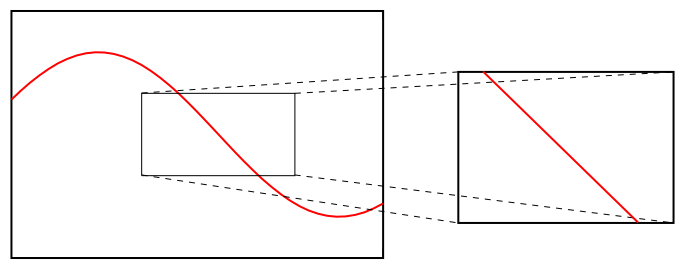
\includegraphics[width=0.5\textwidth]{microaffinity}
  \end{center}

  \vspace*{-2em}
  \begin{varblock}{10.8cm}{The axiom of microaffinity}
    \justifying
    Let~$\Delta = \{ \varepsilon \in \RR \,|\, \varepsilon^2 = 0 \}$.
    For any function $f : \Delta \to \RR$,
    there is a unique number~$a \in \RR$ such that
    $f(\varepsilon) = f(0) + a \varepsilon$
    for all~$\varepsilon \in \Delta$.
  \end{varblock}

  \vspace*{-1em}
  \small
  \begin{itemize}
    \item The \hil{derivative} of a function~$f : \RR \to \RR$ at~$x_0 \in \RR$
    is the unique number~$a \in \RR$ such that~$f(x_0 + \varepsilon) = f(x_0) +
    a \varepsilon$ for all~$\varepsilon \in \Delta$. \\[-1.2em]
    \item Manifolds are \hil{just sets}. \\[-1.2em]
    \item A \hil{tangent vector} to~$M$ is a map~$\Delta \to M$.
  \end{itemize}

  \jnote{1}{Differential geometry abounds with intuition which can't be
  formalized in the standard account of differential geometry. For instance, we
  can't literally define a tangent vector to be an infinitesimal piece of a
  curve -- we have to resort to germs of smooth functions or derivations --
  or speak about infinitesimal deformations of the identity transformation.

  Synthetic differential geometry was born to provide an account of
  differential geometry which is both rigorous and closer to intuition than the
  standard account. Its starting point is the axiom of microaffinity, which is
  very useful but wildly false in classical mathematics. The fundamental
  theorem about synthetic differential geometry, connecting it with the
  ordinary world of smooth manifolds, is that there exist \emph{well-adapted
  models} for synthetic differential geometry -- toposes~$\E$ such that:
  \begin{enumerate}\justifying
    \item There is a functorial way of associating to any smooth manifold~$M$
    an object~$y(M)$ of~$\E$ (something which~$\E$ believes to be a set) and
    to any smooth map~$f : M \to N$ a morphism~$y(f) : y(M) \to y(N)$ of~$\E$
    (something which~$\E$ believes to be map).
    % (item is referenced below by number)
    \item Any morphism in~$\E$ of type~$y(M) \to y(N)$ is
    of the form~$y(f)$ for a smooth map~$f$, and if~$\E \models y(f) = y(g)$,
    then actually~$f = g$.
    \item In~$\E$, the axiom of microaffinity and related axioms hold for the
    ring~$y(\RR^1)$.
  \end{enumerate}}

  \jnote{2}{Here are two examples for synthetic reasoning and synthetic
  constructions.

  \begin{itemize}\justifying
    \item We can compute the derivative of~$f$ with~$f(x) = x^2$ as follows:
    For all~$\varepsilon \in \Delta$, $f(x + \varepsilon) = (x + \varepsilon)^2
    = x^2 + 2x\varepsilon$, hence~$f'(x) = 2x$ by the definition on the slide.

    \item Write~``$M^\Delta$'' for the set of all maps~$\Delta \to M$. A
    \emph{vector field} on a manifold (set)~$M$ is just a map~$X : M \to
    M^\Delta$ such that~$X(p)(0) = p$ for all~$p \in M$. A tangent field~$X$
    induces an infinitesimal path~$\gamma : \Delta \to M^M$ in the space (set)
    of transformations of~$M$, by setting~$\gamma(\varepsilon) = (p \mapsto
    X(p)(\varepsilon))$.

    Conversely, a path~$\gamma : \Delta \to M^M$ such that~$\gamma(0) =
    \mathrm{id}_M$ yields a vector field~$X : M \to M^\Delta$ by setting~$X(p) =
    (\varepsilon \mapsto \gamma(\varepsilon)(p)$. No continuity or smoothness
    checks have to be carried out.
  \end{itemize}

  There are also notions in synthetic differential geometry which
  don't have a classical counterpart. For instance, in synthetic differential
  geometry it's possible to view differential forms on~$M$ -- which are usually
  thought of as \emph{functionals} on (exterior powers of) the tangent bundle
  -- as \emph{quantities} (maps from~$M$ into a certain nonclassical object).}

  \jnote{3}{Recall the following standard reflection principle taught in
  undergraduate calculus: Even though continuity is officially a property which
  depends only on the input/output behaviour of a function, reflecting on the
  \emph{term} used to define a given function often allows us to quickly
  conclude that it's continuous. For instance, any function defined by a
  polynomial expression is continuous.

  Synthetic differential geometry yields a new reflection principle, for
  ordinary manifolds, which improves both on the assumption and on the
  conclusion: Any map between manifolds which is definable in constructive
  mathematics (so in particular, any map which is given by a polynomial
  expression) is smooth (so in particular continuous). This is due to item~2
  above.

  Synthetic differential geometry is very well-developed and at your disposal.
  References include:
  \begin{itemize}
    \item \fixedhref{...}{Notes for highschool students} (in German)
    \item \fixedhref{...}{...}, a blog post by Andrej Bauer
    \item \fixedhref{...}{...}, a short introduction by ... (Primer)
    \item \fixedhref{...}{...}, the definitive book by Anders Kock
  \end{itemize}

  [Technical comment: The object~$y(\RR^1)$ will usually not be the object of
  Dedekind real numbers in~$\E$.]}
\end{frame}


\section[Commutative algebra]{Applications to commutative algebra}

\begin{frame}{The little Zariski topos of a ring}
  \small\vspace*{-0.8em}
  Let~$A$ be a ring (commutative, with unit). We recursively define
  \[ D(f) \models \varphi \quad \text{(``$\varphi$ holds away from the zeros of~$f$'')} \]
  for~$f \in A$ and statements~$\varphi$. Write
  ``$\Spec(A) \models \varphi$'' to mean~$D(1) \models \varphi$.

  \vspace*{-1em}
  \[\footnotesize\renewcommand{\arraystretch}{1.25}\begin{array}{@{}l@{\ }c@{\ }l@{}}
    D(f) \models \top &\text{iff}& \text{true} \\
    D(f) \models \bot &\text{iff}& \text{$f$ is nilpotent} \\
    D(f) \models x = y &\text{iff}& x = y \in M[f^{-1}] \\
    D(f) \models \varphi \wedge \psi &\text{iff}&
      \text{$D(f) \models \varphi$ and $D(f) \models \psi$} \\
    D(f) \models \varphi \vee \psi &\text{iff}&
      \text{there exists a partition~$f^n = fg_1 + \cdots + fg_m$ with,} \\
    &&\quad\text{for each~$i$, $D(fg_i) \models \varphi$ or $D(fg_i) \models \psi$} \\
    D(f) \models \varphi \Rightarrow \psi &\text{iff}&
      \text{for all~$g \in A$, $D(fg) \models \varphi$ implies $D(fg) \models \psi$} \\
    D(f) \models \forall x\?M^\sim\_ \varphi(x) &\text{iff}&
      \text{for all~$g \in A$ and $x_0 \in M[(fg)^{-1}]$, $D(fg) \models \varphi(x_0)$} \\
    D(f) \models \exists x\?M^\sim\_ \varphi(x) &\text{iff}&
      \text{there exists a partition~$f^n = fg_1 + \cdots + fg_m$ with,} \\
    &&\quad\text{for each~$i$, $D(fg_i) \models \varphi(x_0)$ for some~$x_0 \in M[(fg_i)^{-1}]$}
  \end{array} \]

  \jnote{1}{Irrespective of whether~$A$ is a local ring, its mirror
  image~$A^\sim$ is always a local ring (that is, the axioms of what it means
  to be a local ring hold in~$\Spec(A)$).

  A basic application of the internal language of~$\Spec(A)$ are
  local-to-global principles. For instance:
  \begin{itemize}\justifying
    \item The statement ``the kernel of a surjective matrix over a local ring
    is finite free'' admits a constructive proof. It therefore holds
    in~$\Spec(A)$. Its external meaning is that the kernel of a surjective
    matrix~$M$ over~$A$ is finite locally free (there exists a partition~$1 =
    f_1 + \cdots + f_n$ such that for each~$i$, the localized
    module~$(\operatorname{ker} M)[f_i^{-1}]$ is finite free).

    \item The ring~$A$ is a Prüfer domain if and only if~$A^\sim$ is a Bézout
    domain. Therefore any constructive theorem about Bézout domains entails a
    corresponding theorem about Prüfer domains. Bézout domains are quite rare,
    while Prüfer domains abound (for instance the ring of integers of any
    number field is a Prüfer domain).
  \end{itemize}}

  \jnote{2}{More advanced applications are rendered possible by the observation
  that, if~$A$ is a reduced ring ($x^n = 0 \Rightarrow x = 0$), its mirror
  image~$A^\sim$ is \emph{anonymously Noetherian} (every ideal is \emph{not
  not} finitely generated) and \emph{a field}. This fact doesn't have a
  classical counterpart -- in general, neither~$A$ nor its stalks nor
  its quotients nor its subrings are Noetherian or fields.

  This reduction technique allows to give a new proof of
  Grothendieck's generic freeness lemma which substantially improves on the
  previously known proofs in length and clarity: from approximately three
  pages (requiring several advanced prerequisites in commutative algebra) to a
  single paragraph (requiring only the tiny bit of topos theory needed in order to
  setup the internal language).

  Details are \fixedhref{...}{here} (XXX link Munich slides).

  As mentioned before, any proof involving the internal language can be
  \emph{unwound} to yield a direct proof not referencing toposes. Depending on
  the logical complexity of the statements appearing in the internal proof,
  this process can substantially lengthen the proof. In the case of the new
  proof of Grothendieck's generic freeness lemma, we were lucky to
  \fixedhref{obtain a one-page proof}{...} using this process. (This crucially
  rested on the fact that we were able to eliminate the use of the Noetherian
  property from the internal proof; else the unwound proof would have been much
  longer.)}
\end{frame}


\backupstart

\section[Algebraic geometry]{Applications in algebraic geometry}

\begin{frame}{Understanding algebraic geometry}
  \vspace*{-1.5em}\small
  \begin{varblock}{0.9\textwidth}{}
    \justifying
    Understand \hil{notions of algebraic geometry} over a scheme~$X$ as
    \hil{notions of algebra} internal to~$\Sh(X)$.
  \end{varblock}

  \only<1>{
    \centering
    \rotatebox{90}{\tiny\scalebox{0.8}{Illustration: Carina Willbold}}\hspace{-0.05cm}%
    \includegraphics[width=0.7\textwidth]{external-internal-small}
    \par
  }

  \pause

  \small\centering
  \scalebox{0.83}{\begin{tabular}{ll}
    \toprule
    externally & internally to $\Sh(X)$ \\
    \midrule
    sheaf of sets & set \\
    % sheaf of rings & ring \\
    sheaf of modules & module \\
    % sheaf of finite type & finitely generated module \\
    finite locally free sheaf & finite free module \\
    % coherent sheaf & coherent module \\
    tensor product of sheaves & tensor product of modules \\
    % sheaf of Kähler differentials & module of Kähler differentials \\
    sheaf of rational functions & total quotient ring of~$\O_X$ \\
    dimension of $X$ & Krull dimension of~$\O_X$ \\
    spectrum of a sheaf of~$\O_X$-algebras & ordinary spectrum [with a twist] \\
    % big Zariski topos of $X$ & big Zariski topos of the ring $\O_X$ [with a twist] \\
    higher direct image & sheaf cohomology \\
    \bottomrule
  \end{tabular}}

  \footnotesize

  \begin{columns}[c]
    \begin{column}{0.47\textwidth}
      \begin{exampleblock}{}
        \justifying
        Let $0 \to \F' \to \F \to \F'' \to 0$ be a short exact sequence
        of sheaves of~$\O_X$-modules. If~$\F'$ and~$\F''$ are of finite type,
        so is~$\F$.
      \end{exampleblock}
    \end{column}

    \begin{column}{0.1\textwidth}
      \vspace*{1.1em}
      \scalebox{3}{$\Leftarrow$}
    \end{column}

    \begin{column}{0.44\textwidth}
      \begin{exampleblock}{}
        \justifying
        Let~$0 \to M' \to M \to M'' \to 0$ be a short exact sequence of
        modules. If~$M'$ and~$M''$ are finitely generated, so is~$M$.
      \end{exampleblock}
    \end{column}
  \end{columns}
\end{frame}

\begin{frame}{Synthetic algebraic geometry}
  Usual approach to algebraic geometry: \hil{layer schemes above ordinary set theory}
  using either
  \begin{itemize}
    \item locally ringed spaces
    \small
    \begin{multline*}
      \text{set of prime ideals of~$\ZZ[X,Y,Z]/(X^n+Y^n-Z^n)$} + {} \\
      \text{Zariski topology} + \text{structure sheaf}
    \end{multline*}
    \normalsize
    \item or Grothendieck's functor-of-points account, where a scheme is a
    functor~$\Ring \to \Set$.
    \small\[ A \longmapsto \{ (x,y,z) \in A^3 \,|\, x^n+y^n-z^n=0 \} \]
  \end{itemize}
  \bigskip

  \hil{Synthetic approach:} model schemes \hil{directly as sets} in
  the internal universe of the \mbox{\hil{big Zariski topos}} of a base scheme.
  \small
  \[ \{ (x,y,z) \? (\affl)^3 \,|\, x^n+y^n-z^n=0 \} \]
\end{frame}

\backupend

\end{document}
